% Being section ----------------------------------------------------------------
\section{Introduction}

% General introduction ---------------------------------------------------------
\begin{frame}{Welcome}

    \begin{figure}[ht]
        \centering
        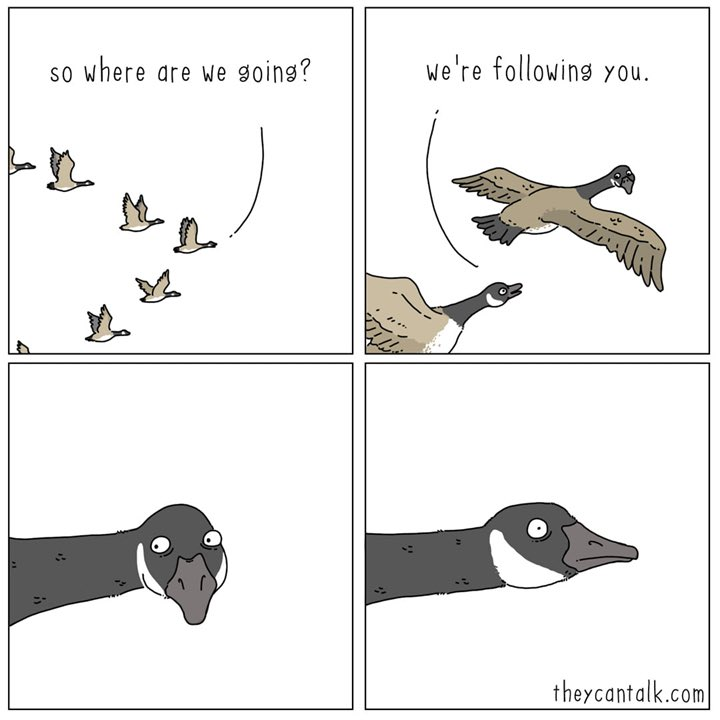
\includegraphics[width=0.5\linewidth]{./resources/meme-birds.jpeg}
    \end{figure}
    
    Welcome to the P218 - Econometrics I TA sessions!
    \begin{itemize}
        \item \textbf{Email:} gsimoesgaspar@london.edu / gabrielsgaspar@gmail.com
        \item \textbf{Office:} P320 Plowden Building
    \end{itemize}
    
\end{frame}

\begin{frame}{Admin}

    \textbf{Tutorials:} Fridays from 12:45h to 15:30h London time.
    \begin{itemize}
        \item \textbf{Frequency:} Usually the week you have a problem set due. I will email you at the start of the week confirming the location.
        \item \textbf{Format:} In person discussion / presentation. If there are any topics you want me to emphasize, please let me know before the session.
    \end{itemize}
    
    \vspace{2em}
    
    \textbf{Problem Sets:} Due after every two sessions.
    \begin{itemize}
        \item \textbf{Hand in:} Submit self-contained PDF with answers, figures and tables (use \LaTeX).
        \item \textbf{Code:} Some code will be required for problem sets (not loads). Please hyperlink link to your Github repository with code.
        \begin{itemize}
            \item E.g. "The code for the following question can be found in this \href{https://github.com/gabrielsgaspar/P218-Econometrics}{\underline{Github repo}}."
        \end{itemize}
    \end{itemize}

    \vspace{2em}
    
    \textbf{Final exam:} Scheduled for December 16 from 16:00h to 19:00h.
    
\end{frame}
\begin{frame}{Advice}

    This is a PhD level course, so take it seriously.
    \begin{itemize}
        \item Alexey will cover a lot of material and in great detail. It is perfectly fine if you don't understand everything in lecture.
        \item Look at different reference books if things are not clear.
        \item Feel free to email me with questions - I will try my best to help you.
    \end{itemize}

    \vspace{2em}
    
    Problem sets are lengthy.
    \begin{itemize}
        \item Start early. One week is not enough to properly complete a problem set (especially the later ones).
        \item Make sure you understand the concepts being covered.
    \end{itemize}
    
\end{frame}